% :autocmd BufWritePost * !pdflatex thesis.tex
\documentclass[a4paper,11pt]{kth-mag}
\usepackage[T1]{fontenc}
\usepackage{textcomp}
\usepackage{lmodern}
\usepackage[utf8]{inputenc}
\usepackage[swedish,english]{babel}
\usepackage{modifications}
\usepackage{amsmath}
\usepackage{amsfonts}
\usepackage{listings}
\usepackage{alltt}
\usepackage{subfigure}
\usepackage{draftwatermark}
%\usepackage[firstpage]{draftwatermark}

\SetWatermarkLightness{0.9}
\SetWatermarkScale{1.1}

\usepackage{tikz}
\usetikzlibrary{automata,positioning,shapes.symbols}

% prevent latex from splitting footnotes over multiple pages
% http://www.tex.ac.uk/cgi-bin/texfaq2html?label=splitfoot
\interfootnotelinepenalty=10000

\newcommand{\todo}[1]{\textbf{todo: #1}}
\newcommand{\rephrase}{\textbf{(rephrase)} }

\title{Test-inspired runtime verification}

\subtitle{Using a unit test-like specification syntax for runtime verification}

\foreigntitle{"TODO: Test-inspirerad runtime-verifiering"}

\author{Adam Renberg}
\date{May 2012}
\blurb{Master's Thesis at CSC\\Supervisor Valtech: title? Erland
Ranvinge\\Supervisor CSC: title Narges Khakpour\\Examiner: title Johan Håstad}
\trita{TRITA xxx yyyy-nn}

\begin{document}

\lstset{
	basicstyle=\ttfamily,
	keywordstyle=\bfseries,
	commentstyle=\color{gray},
	columns=fixed,
	tabsize=2,
	showspaces=false,
	showstringspaces=false,
	numbersep=20pt}

\frontmatter
\pagestyle{empty}
\removepagenumbers
\maketitle
\selectlanguage{english}




%================================================
%====== The Abstracts
%================================================

\begin{abstract}

Abstract in English. Write when most of the report is written.

\bigskip\noindent
Keywords: Runtime Verification, Unit Testing, Program Correctness
\end{abstract}
\clearpage

\begin{foreignabstract}{swedish}

Sammanfattning på svenska. Skrivs sist.

\bigskip\noindent
Keywords (Sökord? Nyckelord?):
\end{foreignabstract}
\clearpage




%================================================
%====== The Preface and ToC
%================================================

\pagestyle{newchap}
\chapter*{Preface}

This is a master thesis / degree project in Computer Science at the Royal
Institute of Technology (KTH), Stocholm. The work was done at Valtech Sweden,
an IT Consultancy. It was supervised by Erland Ranvinge (Valtech) and Dr.
(\todo{check}) Narges Khakpour (CSC KTH).

\todo{Thanks to people.}. Narges, Erland. Valtech. Proof readers.

Any errors contained in the report are mine and mine alone \rephrase.
\clearpage

\pagestyle{newchap}
\tableofcontents*
\mainmatter




%================================================
%====== Chapter 1, Introduction
%================================================

\pagestyle{newchap}
\chapter{Introduction} \label{chapter-introduction}

Due to the increasing size and complexity of computer software it has become
increasingly difficult, if not impossible, to convince oneself that the
software works as desired. This is where verification tools can be used to
great effect. Of these tools, testing is the one familiar to most developers,
and in widespread use. The introduction of agile development practices and
test-driven development has also popularized the concept of \textit{unit
testing}, in which small modules of a program or system are tested
individually.

While testing is popular and often works well, it is incomplete and informal,
and thus yields no proof that the program does what it should - i.e. follows
its specification. Formal verification techniques, such as theorem proving,
model checking (and its bounded variant), can give such proofs. However, they
suffer from complexity problems (\textit{incompleteness},
\textit{undecidability}) and practical issues, such as the so-called
\textit{state explosion} problem. Often they cannot be fully automated.

A relatively new approach in this area is runtime verification, in which the
program \textit{execution} is verified against its specification. With the
specification written in a suitably formal language, the program can be given a
mathematical proof that its specification is followed.


\section{Problem Statement} \label{section-problem-statement}

How can runtime verification specifications be written in a manner that uses
the syntax of the target program's programming language, and resembles
the structure of unit tests?


\section{Motivation}

Checking that a program works correctly is of great interest to software
developers. Formal verification techniques are helpful, but as mentioned above,
traditional methods can be impractical with larger programs, and verification
by testing is informal and incomplete. Runtime verification can here be a
lightweight addition to the toolbox of verification techniques.

The specification languages used by runtime verification approaches are often
based on formal languages/formalisms (e.g.\ logic or algebra) and not written
in the target program's programming language. This means that writing the
specifications requires specific knowledge and expertise in mathematics. It
also requires mental context-switching, between writing the program and writing
the specification, and special tools to support this specialised language's
syntax.

In contrast, unit testing frameworks often utilise the programming language to
great effect, and they are a common part of the software development process.

If runtime verification specifications more resembled unit tests, and were
written in the target program's programming language, it might popularise the
use of runtime verification for checking the correctness of programs.



\section{Disposition}

The first time an important concept is introduced it is written in
\textit{italics}. These words are briefly explained in
Appendix~\ref{appendix-dictionary}.

The rest of this report is structured as follows.
Chapter~\ref{chapter-background} gives a
background to the subject of verifying program correctness.
Chapter~\ref{chapter-previous-research} continues
by describing the previous research on runtime verification and the syntax of
specification languages. It also gives an overview of the current ideas in unit
testing.

Chapter~\ref{chapter-approach} describes the approach this work takes to
solving the problem stated in Section~\ref{section-problem-statement}. It
describes the syntax, instrumentation and verification techniques used in a
proof-of-concept implementation, and gives a formal foundation to a subset of
the syntax. Chapter~\ref{chapter-evaluation} then gives an evaluation of this
work...
\todo{}.

Conclusions and a discussion of this and future work is done in
Chapter~\ref{chapter-conclusions}.





%================================================
%====== Chapter 2, Background
%================================================

\pagestyle{newchap}
\chapter{Background} \label{chapter-background}

Runtime verification is a new area of research, but the research on
verification and formal approachs goes back several decades. Research of interest
include the early work on formal methods, e.g.\ by Hoare \cite{hoare69} and
Floyd \cite{floyd67}, and work on logics suitable for runtime verification,
e.g. LTL by Pnueli \cite{pnueli77}. The seminal work done by Hoare, Floyd and
Pnueli lay the foundation for many interesting approaches. LTL is one of the
common formal languages used for specifications in runtime verification.

This chapter gives a short overview of the background to the concepts of this
report. It starts with laying out what we mean by proving the correctness of
programs in Section~\ref{section-proving-correctness}. Section~\ref{section-rv}
describes runtime verification and its place in proving correctness. And
finally, Section~\ref{section-testing} discusses testing - syntax, style and
other concepts.


\section{Proving Correctness} \label{section-proving-correctness}

A correctness proof is a certificate, based in mathematics and logics, that a
program/system/function follows its specifications, i.e.\ does what it is
supposed to do. There are several approaches, with their respective advantages
and disadvantages.

\textit{Theorem proving}, as started by Hoare \cite{hoare69}, Floyd
\cite{floyd67} and others, is the manual, semi-automated, or (not so often)
fully automated process of mathematically proving that the system follows its
specification. There are many ways of doing such proofs.

One way is to prove that at all points in the program, given inputs satisfying
some pre-conditions, the outputs will satisfy the post-conditions. By
formulating post-conditions for the exit point(s) of the program so that they
follow the specification, and by linking together the pre-conditions of program
points with their preceding program points' post-conditions, we know that
correct indata will yield correct results.

This way of proving correctness often yields the best results \rephrase. But it
is slow, hard to automate, and therefore requires much manual work. Wading
through large programs thus often becomes impractical.

\textit{Model checking} is the concept of verifying that a \textit{model} of a
system (the \textit{system model}) follows its specification. This requires
that both the model and the specification is written in a mathematical
formalism. Given this, the task becomes to see if the model satisfies the
logical formula of the specification. It is often simpler than theorem proving,
and can be automated.

The model of the system is usually structured as a finite state machine (FSM),
and verification means visiting all accessible states, checking that they
follow the specification (which also can be represented as an FSM). This can be
problematic, especially when the state space becomes very big, something known
as the \textit{state explosion problem}. There are approaches to address this
issue, such as \textit{bounded model checking}, or by using higher-level
abstractions.

Proving that a model of a system is correct can be very useful, but it suffers
from the inherent flaw of only verifying the model, not the actual system. The
model can be difficult to construct, or deviate too far from the system. It can
not take the dynamic properties and configuration of the executing code into
account.

Runtime verification attempts to solve this by dealing directly with the
system, creating its model at runtime.


\section{Runtime Verification} \label{section-rv}

Runtime verification (RV) is a dynamic approach to checking program
correctness, in contrast to the more traditional formal static analysis
techniques discussed above.

Runtime verification aspires to be a light-weight formal verification
technique, see e.g.\ \cite{leucker09abriefaccount,delgado04taxonomy}. It
verifies whether properties of a specification hold \textit{during the
execution} of a program.

The specification that should be verified is often written in a formal
language, a logic or a calculus, such as linear temporal logic \cite{pnueli77}.
To build a system model for verifying the properties of the specification, the
target program needs to emit or expose certain events and data. The collected
events and data are used to build the system model. RV frameworks typically
use \textit{code instrumentation} to generate \textit{monitors} for this end.

A monitor is either just part of a recording layer added to the program, which
stores the events and data needed for verification, or also the part of the
machinery that performs verification.

There are two types of verification: \emph{online} and \emph{offline}. In
online verification, the analysis and verification is done during the
execution, in a synchronous manner with the observed system. In offline
verification, a log of events is analysed at a later time. Online verification
allows actions to be taken immediately when violations against the
specifications are detected, but with considerable performance cost. Offline
verification only impacts the performance by collecting data.

When a violation of the specification occurs, simple actions can be taken
(e.g.\ crash the program, log the error, send emails, etc.), or more complex
responses initiated, resulting in a \textit{self-healing} or
\textit{self-adapting} system (see e.g.\ \cite{huebscher08survey}).

Relevant work on runtime verification include \cite{bauer06monitoring}, in
which Bauer et al.\ use a three-valued boolean logic (true, false and ?) to
reflect that a specification can not only be satisfied (true) or violated
(false), but also neither yet, or, in the future it may be either. Bauer et
al.\ also show how they transform specifications into automata (which they call
\textit{runtime monitors}).

Bodden presents in \cite{bodden05efficientrv} a framework for RV implemented
through \emph{aspect-oriented programming} using
\textit{aspectj}\footnote{\texttt{http://www.eclipse.org/aspectj/}} in Java,
with specifications written as code annotations. Aspect-oriented programming is
described in more detail in Section~\ref{section-aspects}.

Leucker et al.\ present a definition of RV in \cite{leucker09abriefaccount},
together with an exposition of the advantages and disadvantages, similarities
and differences, with other verification approaches. In
\cite{delgado04taxonomy}, Delgado et al.\ classify and review several different
approaches and frameworks to runtime verification.


\section{Testing} \label{section-testing}
On the other end of the program-correctness-checking spectrum is
\emph{testing}, which is the practical approach of checking that the program,
given a certain input, produces the correct/acceptable output. Testing is not
complete (for all but the most trivial programs, it is impossible to write
complete tests), and lacks a formal foundation, so it cannot be used for formal
verification. Testing can be a complement to more formal techniques, such as
RV. It is in many cases the sole correctness-checking tool.

\textit{Unit testing} is the concept of writing small tests, or test suites,
for the units in a program, such as functions, classes, etc. These tests are
used during development to test the functionality of the units. The aim is to
reduce the risk of breaking existing functionality when developing new
features, or modifying existing code, by preventing regression.

Unit testing is quite young, perhaps having begun in earnest in the 90s, and it
was popularized by the extreme programming (XP)
movement\footnote{\texttt{http://www.extremeprogramming.org/}}. Testing in
general is very old.

Kent Beck introduced the style of the modern unit testing framework in his work
on a testing framework for Smalltalk \cite{becksmalltalktesting}. Together
with Eric Gamma he later ported it to Java, resulting in
\textit{JUnit}\footnote{\texttt{http://www.junit.org/}}.
Today, this has lead to frameworks in several programming languages, and they
are collectively called xUnit \cite{fowlerxunit}.

Writing unit tests, often using unit testing \textit{frameworks} such as JUnit
for Java and
\textit{unittest}\footnote{\texttt{http://docs.python.org/library/unittest.html}}
for Python, is a common practice on many development teams.

Testing is often a manual process, taking up a large part of development time
(see e.g.\ \cite{brooks75mythicalmanmonth}). Still, there are tools to
automatically generate tests.

When discussing testing, and unit testing in particular, we must mention the
concept of test-driven development (TDD). Also made popular by XP, it consists
of the cycle: (1) write a failing test, (2) make it pass by writing the
simplest code you can, and (3) refactor - rewrite the code so that it becomes
good. Tests here play the part of specifications for the units of the program.





%================================================
%====== Chapter 3, Previous Research
%================================================

\pagestyle{newchap}
\chapter{Previous Research} \label{chapter-previous-research}

As we saw in Section~\ref{section-rv}, runtime verification is a technique for
verifying a program's compliance against a specification during runtime. These
specifications need to be written somehow, which will be discussed in
Section~\ref{section-specifications}. Approaches for verification are discussed
in Section~\ref{section-verification}. For verification to work, during
runtime, the program usually needs to be instrumented in such a way that the
verification process can access all pertinent data. This is discussed in
Section~\ref{section-instrumentation}

The design of unit test syntax is discussed in
Section~\ref{section-unit-testing}. The combination of the two, runtime
verification and unit testing, will be the main subject in
Chapters~\ref{chapter-approach} and~\ref{chapter-evaluation}.


\section{Specifications} \label{section-specifications}

Specifications come in many forms, from the informal ones like ``I want it have
cool buttons'', to the contractual ones written between companies and their
clients, to tests, and to formal specifications, written in formal languages,
specifying properties that should verifiably hold for the program. It is these
last two types of specifications that we are interested in here, and which play
an important role in runtime verification.

In general, specifications should be abstract, written in a high-level
language, and succinctly capture the desired property. Writing erroneous
specifications is of course a possibility; specifications need to be easier for
humans to verify than the program's implementation. There is little point in
having a specification as complex as the program itself, except for as a point
of reference. A program can be seen as an all-encompassing, perfect,
always-true, specification of itself.


\subsection{Formalisms for Specifications}

There are several common formalisms for writing specifications, and many papers
that expand, rephrase and illuminate on them. Although they can be quite
different, they share a common origin in the work done by Floyd \cite{floyd67},
Hoare \cite{hoare69}, and others before them.  Floyd thought of formulas
specifying in/out properties of statements, and chaining these together to form
a formal proof for the program. Hoare elaborated on this idea by basing his
proofs on a few axioms of the programming language and target computer
architecture, and building the proof from there.


\subsubsection{Linear Temporal Logic}

Linear Temporal Logic (LTL) was first discussed by Pnueli in \cite{pnueli77},
and has since been popular in many areas dealing with a system model containing
a temporal dimension. As Pnueli describes it, it is simpler than other logics,
but expressive enough to describe many problems of interest for verification.
This has been affirmed by the diverse use of LTL by many researchers.

LTL uses a system model of \textit{infinite execution traces}, or
\textit{histories}, of the states of the execution. LTL specifications are
formulas that operate on these states. An LTL formula consists of
\textit{propositional variables} that work on the domain model of the state
(checking variables, inputs, global state, etc.), the normal logical operators
such as negation and disjunction, and some temporal operators. The most basic
and common temporal operators are $\boldsymbol{X}$, \textit{next}, and
$\boldsymbol{U}$, \textit{until}. Other operators can be derived from these,
such as $\boldsymbol{G}$, \textit{globally}, and $\boldsymbol{F}$,
\textit{eventually}.

An example LTL formula, taken from a list of common specification patterns
\cite{dwyer99patterns}, could be: $S$ precedes $P$, i.e.\ if the state $P$
holds sometime, the state $S$ will hold before it. This is shown in
Figure~\ref{figure-ltl}.

\begin{figure}[h!]
	\[
	\boldsymbol{G} \, P \rightarrow (\neg P \, \boldsymbol{U} \, (S \wedge \neg P)
	\]

	\caption{An example of an LTL formula. This can be read as: Globally, if $P$
	holds, then, before $P$, $S$ held at some point.}
	\label{figure-ltl}
\end{figure}

In \cite{bauer06monitoring} Bauer et al.\ introduce a three-valued boolean
semantics for LTL, calling it LTL$_3$, which takes the values (true, false and
?).  This logic is arguably more suited for the finite nature of runtime
verification, whereas LTL was designed with infinite traces in mind. The
semantics of LTL$_3$ reflect the fact that when verifying runtime verification
specifications, the result can not only be that the specification is satisfied
or violated; it can be inconclusive as well. For satisfied or violated
specifications, no further verification is required - we already know the
outcome. For inconclusive results, we need to continue with the verification,
as, with future events, the result could change into either satisfied or
violated.

There is a counterpart to LTL in the real-time setting called Timed Linear
Temporal Logic (TLTL). It introduces clocks to make specifications
of real-time properties possible. It is of great interest to runtime
verification, but will not be discussed further here. See e.g.\
\cite{bauer06monitoring} for more.


\subsubsection{Design by Contract}

Design by Contract was introduced by Bertrand Meyer in
\cite{meyer92applyingdbc}, and has been fully implemented in the Eiffel
programming language. A contract is the idea that functions, and methods on
objects, promise to fulfill certain post-conditions (or promises) if the inputs
they are given fulfill the pre-conditions (or requirements) specified in the
contract.  Design by Contract also contains constructs for specifying
loop-invariants and class-invariants, properties that should always hold during
loops and for objects of a class, respectively. Assertions (see below) are also
usually available.

Design by Contract is inspired by Hoare logic, and is essentially Hoare logic
written in a certain style.


\subsubsection{Assertions}

A common construct that is part of many popular programming languges, like C,
Java and Python, is the \texttt{assert} statement. It is a way to state that
some predicate should hold at a point in the program. Usually the predicate is
an expression in the programming language, and is not supposed to alter the
program state.

Assertions are distinct from the normal program flow, and not to be conflated
with exceptions. Assertions check for properties that should always be true,
anything else would be a programming error.


\subsection{Writing Specifications}

For verification in general, specifications can be written and used externally
to the program. They can be used in specialized model-checking tools, in tools
for theorem proving, etc.

Runtime verification requires that the specifications are accessible when
building and running the program. At the very least, the program needs to be
instrumented to expose the correct system model so that the specification can
be verified. It is sometimes desired in runtime verification to do online
verification, and then the specifications need to be available and embedded
into the system. A few different approaches have been tried to support this.

Approaches to writing specifications can be divided into two parts: those that
require you to manually mark code for verification, and those that inject the
verification code from external specifications.

Rosuenblum \cite{rosenblum95practicalassertions} uses specially annotated
comments, written directly in the code. Bodden \cite{bodden05efficientrv} uses
Java annotations, which are written at function and variable definitions, to
mark code for verification. The programming language Eiffel has full language
support for Design by Contract, with pre- and post-conditions, invariants, and
more. These are written in direct proximity to the code to be verified. For
simple cases it is common to write assertions in the program
\cite{bartetzko01jass}.

Other approaches, such as the ones taken by Jalili et al.\ in
\cite{jalili07rverl} and Barringer et al.\ in \cite{barringer03eagle}, use
external specification files.



\section{Verification against Specifications} \label{section-verification}

Specifications for runtime verification are written so that programs can be
verified against them - to see whether they follow the specification, or
violate parts of it.

There are several ways to verify a program against its specification. A common
one, used in
\cite{bauer06monitoring,bodden05efficientrv,jalili07rverl,barringer03eagle}
among others, is to generate state machines from the specification. These state
machines, sometimes called \textit{runtime monitors}, operate with the input
language of events emitted by the program.

\todo{Write more on this.}


\section{Code Instrumentation} \label{section-instrumentation}

For verification to work, the verifier needs access to events happening in the
program. Such events can be functions called, statements executed, variables
assigned, etc., depending on the system model of the specification language.
The program needs to be instrumented for it to emit such events. This often
means wrapping function calls and variable assignments in a ``recording
layer'', which performs the desired action after logging the event. The events
can then be passed on to the verification tools.

There are four major approaches used for program instrumentation.


\subsection{Pre-processing the Code}

Rosenblum \cite{rosenblum95practicalassertions} uses a pre-processor step in
the C compilation setup to instrument code, where the specifications (called
assertions by Rosenblum) are transformed from comments into regular C code. The
verification code is then compiled together with the program.


\subsection{Post-processing the Code}

It is also possible to rewrite the compiled program, instrumenting the code
after compilation. This way, the program needs no knowledge of the verification
framework. Depending on the compiled objects, this can be more or less
difficult. Binary executables and intermediate formats, such as Java Bytecode
or Common Intermediate Language for the Common Language Infrastructure used by
.Net, require somewhat different approaches.


\subsection{Dynamic Code Rewriting}

In many dynamic languages, such as Python, Ruby or Javascript, it is possible
to rewrite the code during runtime, which is sometimes called \textit{monkey
patching}. A function to be monitored could be rewritten, adding a lightweight
wrapper that records all calls to it, and then passes on the call to the actual
function.


\subsection{Aspects} \label{section-aspects}

An interesting approach to code instrumentation is to use aspect-oriented
programming. In aspect-oriented theory, a program should be divided into
modules, each only dealing with their own \textit{concern}. Logging, however,
is a \textit{crosscutting concern}, as it is used by several unrelated modules.
The goal is to not scatter logging code across the modules, and to not tangle
it with the modules' own logic. This can be done by defining the logging code
as \textit{aspects}, which consists of the logging code, called the
\textit{advice}, and a \textit{point cut}, which is a formula describing when
the advice should be executed. The possible execution points for a point cut
are called \textit{join points}.
AspectJ\footnote{\texttt{http://www.eclipse.org/aspectj/}} is the canonical
framework for aspect-oriented programming.

Runtime verification is a typical case of a cross-cutting concern. Bodden
\cite{bodden05efficientrv} uses AspectJ in his runtime verification
implementation.

Aspects in AspectJ are implemented as a post-processing step in the compilation
process, adding wrapper code for handling the aspects.


\section{Unit Testing} \label{section-unit-testing}

We discussed testing and unit testing in general in
Section~\ref{section-testing}. Here we'll discuss how it works, and what the
syntax is like.


\subsection{xUnit}

The xUnit style of unit testing \cite{fowlerxunit} has given rise to unit
testing frameworks for many programming languages. Their structure are all
based on the same concept, and since JUnit is the canonical implementation, and
one of the first, implementation, we will use it for a short demonstration. See
Figure~\ref{figure-junit}.

\begin{figure}[h!]
	\begin{center}
	\begin{minipage}{0.7\textwidth}
		\lstset{language=Java}
		\lstinputlisting{figures/junit_example.java}
	\end{minipage}
	\end{center}
	\caption{An example of unit testing syntax, written as a test case for JUnit.}
	\label{figure-junit}
\end{figure}

In JUnit, and xUnit, you run a \textit{test suite} of \textit{test cases},
which contain tests. The example in Figure~\ref{figure-junit}, the test suite
is implicitly created by JUnit, although it is possible to create it and
control it your self. A \textit{test runner} runs the test suite, reporting
progress to the user.  When the tests are finished, any errors are displayed.

In the example in Figure~\ref{figure-junit} has two tests, and methods to set
up and tear down the tests \textit{fixture}. These functions are usually called
\textit{setUp} and \textit{tearDown}, respectively, and are called before and
after each test. The fixture is the surrounding set of objects (environment)
that the object under test requires to work properly.

Test written in this style are traditional unit tests.


\subsection{Mocking and Faking}

A common issue when writing unit tests is that, to instantiate some object X,
or to call some function Y, the program needs access to some other
objects/data/configuration Z. Z might be something simple, which we can easily
create in the test. It might also be a network or database connection, or
something doing heavy calculation, or just something complex.

One way to work around this is to create fake/mock/dummy objects. A fake
network connection has the same interface as a real network connection, but
calling it does not actually transmit anything anywhere, and it might return
pre-defined, hard coded data. Fake objects could save what actions are taken
upon them, and the test could then verify that these are according to
expectations.


\subsection{Expectations}

Instead of writing fake objects, we can create a mock object and pre-record
what actions we expect to be taken upon them. This is called writing
\textit{expectations} \cite{fowler07expectations}. A simple example of
expectations is shown in Figure~\ref{figure-expectations}.

\begin{figure}[h!]
	\begin{center}
	\begin{minipage}{0.7\textwidth}
		\lstset{language=Java}
		\lstinputlisting{figures/expectations_example.java}
	\end{minipage}
	\end{center}

	\caption{An example of expectations, written using jMock and JUnit.
	Example taken from \cite{fowler07expectations}.}
	\label{figure-expectations}
\end{figure}

Figure~\ref{figure-expectations} shows a test of a fictional shop. The test
tests only one thing, the fill method of the Order object, but it requires a
Warehouse object, for access to the inventory. We supply a mock Warehouse, with
expectations on which methods should be called on it, with which arguments and
what they should return.

An expectation follows a simple pattern:

\begin{itemize}
	\item A function, with an optional object, which is expected to be called.
	\item An invocation count of how often the function is expected to be called.
	\item Expected arguments for the function call. These can be explicit values,
		or generic types, or rules defining the acceptable values.
	\item The return value and modifications to the global state; what should
		happen when the function is called.
	\item When the function call should happen, e.g.\ in what sequence of
		function calls, in what global state.
\end{itemize}

There are two common ways of specifying expectations: recording and explicit
specification. Figure~\ref{figure-expectations} shows an example of how to
explicitly specify expectations.

When recording expectations, you create a mock object and call the expected
functions, with expected arguments and return values, in the expected order.
Then you set the mock into replay mode, and it will replay the recorded
expectations, and verify that they occur correctly.

There are several frameworks for working with expectations, such as
jMock\footnote{\texttt{http://www.jmock.org/}} for Java, Rhino
Mocks\footnote{\texttt{http://ayende.com/wiki/Rhino+Mocks.ashx}} for .Net and
Ludibrio\footnote{\texttt{https://github.com/nsigustavo/ludibrio/}} for Python.





%================================================
%====== Chapter 4, Approach
%================================================

\pagestyle{newchap}
\chapter{Approach} \label{chapter-approach}

This chapter describes the proof-of-concept implementation of this report.


\section{Introduction}

As stated in Section~\ref{section-problem-statement}, the objective of this
thesis is to investigate whether it is possible to do runtime verification with
specifications written in the target program's programming language, structured
similar to unit tests. To find a solution for this, there are four issues we
need to address:

\begin{enumerate}
	\item How should the syntax for the specifications be defined, so that it
		looks similar to that of unit tests, but works for runtime verification?
		Which language should be used? Which unit testing framework to take
		inspiration from?
	\item How should the program be instrumented to monitor the system, to expose
		the appropriate events and data, and to build the system model?
	\item How will this be used to verify the system against the
		specification? Online or offline verification? E.g.\ which techniques
		should be used to verify the monitored system against the specification?
	\item How can the resulting approach be provided with a formal foundation?
\end{enumerate}

This report is a documentation on how to solve these issues. The following
sections are each dedicated to one issue, and shows a proof-of-concept of these
ideas. The implementation, called \textit{pythonrv}, can be found
online\footnote{\texttt{https://github.com/tgwizard/pythonrv}}.


\subsection{Definitions}

Here follows some definition that will be used in the following sections.

\begin{itemize}
	\item A \textit{specification} is an construct that determines the correct
		behaviour of a program. It could be a document, describing the programs
		functionality, or a set of inputs and outputs, describing the correct
		results of the program's computation on that set. It could be a reference
		implementation\footnote{For instance, the only specification for python is
		the canonical CPython implementation. Python is defined as ``what CPython
		does''.}. A \textit{formal specification} is a mathematical construct that
		can be used in verification proofs to show that a program works correctly,
		i.e.\ according to its specification.

	\item \textit{Instrumentation} is the act of rewriting, intercepting, or
		patching the program to gain access to its internal state and execution
		flow.

	\item In \textit{pythonrv} a \textit{specification function} is a Python
		function describing a specification, which \textit{pythonrv} can use for
		verification of the program.

	\item A specification function
		\textit{monitors} points (functions) of the program, and the points being
		monitored are called \textit{monitorees}.
\end{itemize}

\subsection{Choice of Language}

During the development of this proof-of-concept, the biggest factor in deciding
what language to use was how it would assist in instrumentation.
Instrumentation is discussed in Section~\ref{section-approach-instrumentation}.
The language should also be in wide use, support quick development, and have an
active testing culture.

Easy access to a non-trivial and actively used system for real-world testing
would be a plus. More on this in Chapter~\ref{chapter-evaluation}.

Python\footnote{\texttt{http://www.python.org}}, among several languages, fits
these criteria, and was chosen as the implementation language.

\section{Syntax} \label{section-approach-syntax}

The canonical framework for doing unit testing in Python is the
\textit{unittest} framework that is included in all modern versions of Python.
Not much development has happened on it in the last years. Many new frameworks
have have spawned, such as PyUnit, Nose and py.test. They build upon the style
of unittest and mostly add new miscellaneous features, such as better test
reporting. The original structure of the unit tests is still prevalent -
unittest builds on the xUnit style of unit testing, discussed in
Section~\ref{section-unit-testing}.

The next section will illustrate the syntax of \textit{pythonrv}.


\subsection{Three Examples}
\lstset{language=Python,numbers=left}

\begin{figure}[h!]
	\begin{center}
	\begin{minipage}{0.7\textwidth}
	\lstinputlisting{figures/syntax_example_1.py}
	\end{minipage}
	\end{center}

	\caption{A specification that monitors the function \texttt{fib} in the
	module \texttt{fibmodule}. The monitored function is, locally to the
specification function, aliased as \texttt{func}. The specification asserts
that the first input to the monitored function is always greater than zero.}
	\label{figure-syntax-example-1}
\end{figure}

The example in Figure~\ref{figure-syntax-example-1} shows the basics of a
\textit{pythonrv} specification, written as a specification function. Line 1
imports the \texttt{rv} module from the \texttt{pythonrv} package. On line 2 it
imports the module containing the function to be monitored. Line 5 defines
the specification as an ordinary Python function called \texttt{spec}, taking
one argument, \texttt{event}. The instrumentation is done line 4 by using the
\textit{function decorator}\footnote{See
Section~\ref{section-approach-instrumentation} for an explanation of function
decorators and \texttt{rv.monitor}.} \texttt{rv.monitor}. \texttt{rv.monitor}
declares that the function \texttt{fib} in \texttt{fibmodule} should be
monitored, and, whenever \texttt{fib} is called, \texttt{spec} should be called
as well.

The specification function itself consists of any valid Python code. It is
passed a special argument, \texttt{event}, which gives the specification
function access to data about the current event. On line 6, the array of input
arguments used to call \texttt{fib} is accessed to check that the first
argument is greater than zero.

The specification function in Figure~\ref{figure-syntax-example-1} will be
called upon every invocation to \texttt{fibmodule.fib}.

\begin{figure}[h!]
	\begin{center}
	\begin{minipage}{0.7\textwidth}
	\lstinputlisting{figures/syntax_example_2.py}
	\end{minipage}
	\end{center}

	\caption{A specification that monitors two functions, \texttt{mymodule.foo}
		and \texttt{mymodule.bar}. It asserts that calls to the two functions
		alternate; that no two calls to \texttt{foo} occurs without a call to
		\texttt{bar} in between, and vice versa. The first call has to be to
		\texttt{foo}.}
	\label{figure-syntax-example-2}
\end{figure}

Figure~\ref{figure-syntax-example-2} shows how a specification function can
monitor two functions. The specification function will be called whenever
either of the monitored functions are called. Which function was called can be
determined from the \texttt{event} argument, as is done on lines 7 and 14. It
is the \texttt{called} attribute of a function in the \texttt{event.fn}
structure that allows for this.

The example also shows how the specification can access a history of previous
events - events that it has handled in the past. \texttt{event.history} is a
list of all events that has occurred that this specification monitors. The last
element is the current event, and the next-to-last element is the previous
element, which can also be accessed as \texttt{event.prev}.

\begin{figure}[h!]
	\begin{center}
	\begin{minipage}{0.7\textwidth}
	\lstinputlisting{figures/syntax_example_3.py}
	\end{minipage}
	\end{center}

	\caption{A more complex example: A specification function that monitors three
		functions, \texttt{foo}, \texttt{bar} and \texttt{baz}, and makes sure that
		\texttt{foo} is called first, then any number calls to \texttt{bar} with
		the first argument as \texttt{True}, and then finally a call to
	\texttt{bar}. After that, any calls are allowed - the specification function
will not be used in verification any longer.}
	\label{figure-syntax-example-3}
\end{figure}

Figure~\ref{figure-syntax-example-3} shows a more advanced example, in which
the \texttt{next} function of the \texttt{event} argument is used.
\texttt{event.next} allows the specification function to add more specification
functions (possibly implemented as closures or lambdas) to be executed when the
next event occurs.

On line 9 the function \texttt{followup} is added to be executed on the next
event. Since \texttt{followup} is added in this way - as a ``oneshot''
specification function - it needs to add itself using \texttt{next} for
verification on subsequent events. This is done on line 22.

Figure~\ref{figure-syntax-example-3} also shows how a specification function
can turn its verification off - i.e. unsubscribe from future events.
\texttt{event.finish} and \texttt{event.success} are essentially the same, and
unsubscribes without further errors. \texttt{event.failure} can be thought of
as a combination of \texttt{event.finish} and \texttt{assert False} (which
always fails).


\subsection{Capabilities and Limitations}

The examples above show the main capabilities of \textit{pythonrv}
specifications. A few minor details were left out, such as how to specify how
much history should be saved for a specification, or how to label
specifications with error levels, so that different actions can be taken
depending on which specification function fails. This is described on the website for
\textit{pythonrv}.


\section{Instrumentation} \label{section-approach-instrumentation}

The previous section showed how \textit{pythonrv} specification functions can
be written. This section will describe how these functions can jack themselves
into the ordinary control flow of the program and gain access to the function
call events and their arguments and associated state.

Instrumentation is done through the \texttt{rv.monitor} \textit{function
decorator} in \textit{pythonrv}. A Python function decorator is similar to
attributes in .Net and annotations in Java. It is essentially a function that
takes in a function and returns a function, possibly modifies it, or uses it in
some way (decorates it) in the processs. This is used throughout Python to, for
instance, turn functions into static or class methods.
Figure~\ref{figure-function-decorator} shows an example function decorator
definition, and Figure~\ref{figure-function-decorator-usages} shows how to use
it.

\begin{figure}[h!]
	\begin{center}
	\begin{minipage}{0.7\textwidth}
	\lstinputlisting{figures/function_decorator.py}
	\end{minipage}
	\end{center}

	\caption{An example of how to define a function decorator.}
	\label{figure-function-decorator}
\end{figure}

\begin{figure}[h!]
	\begin{center}
	\begin{minipage}{0.7\textwidth}
	\lstinputlisting{figures/function_decorator_usages.py}
	\end{minipage}
	\end{center}

	\caption{An example of how to use the function decorator from
	Figure~\ref{figure-function-decorator}.}
	\label{figure-function-decorator-usages}
\end{figure}

\texttt{rv.monitor} first takes arguments specifying what functions should be
monitored, and then the specification function itself.

In Python, almost all\footnotemark\ functions belong to a container of some
sort - a class, an object, or a module. In
Figure~\ref{figure-function-decorator-usages} the functions \texttt{func\_a}
and \texttt{func\_b} belong to the module \texttt{test} (the module's name is
the same as that of the file containing the code). These containers are
essentially dictionaries (\textit{dicts} in Python parlance) of key-value
pairs, where the keys in this case are function names and the values are
objects representing the function code. (There are other types of values in
these containers as well, which we can ignore).

\footnotetext[5]{This is not true of closures - function defined inside other
	functions. These functions cannot be directly referenced or modified from
	outside the defining function. \textit{pythonrv} does not (as of writing)
	support monitoring of closures.}

The instrumentation in \textit{pythonrv} works as follows. First, a wrapper
function is defined for each function to be monitored (for each monitoree).
This wrapper function's main purpose is to call the specifications attached to
the monitored function, and then call the monitored function itself. The
wrapper also does some argument copying and such, to prevent side-effects in
the specifications from interfering with the monitored function. The container
of the monitored function is then extracted, and the reference to the monitored
function is overwritten with a reference to the wrapper. See
Figure~\ref{figure-instrumentation-overview} for an overview.

The implementation of the instrumentation code in \textit{pythonrv} is more
optimized than this - for instance, only ever one wrapper per monitoree is
created, independent of the number of specifications that want to monitor it.

\begin{figure}[h!]
	\begin{center}
	\begin{minipage}{0.7\textwidth}
	\begin{lstlisting}
# rv.py
def monitor(monitorees, specification):
	for monitoree in monitorees:
		# define a wrapper for each monitoree
		def wrapper(*args, **kwargs)
			event = create_event(...)

			# call specification
			specification(event)

			# call the actual function - the
			# monitoree
			return monitoree(*args, **kwargs)

		# overwrite the monitoree in its container
		container = get_container(monitoree)
		setattr(container, monitoree.name, wrapper)
	\end{lstlisting}
	\end{minipage}
	\end{center}

	\caption{An overview of the \textit{pythonrv} instrumentation process,
		written in pseudo-Python. This is just for illustrative purposes and not
		how \textit{pythonrv} actually does the instrumentation.}
	\label{figure-instrumentation-overview}
\end{figure}



\section{Verification} \label{section-approach-verification}

In \textit{pythonrv}, verification is quite simple. The specification functions
are executable, and executing them on the appropriate events, providing access
to the current data, verifies that the specification they represent is
followed.

Specification functions notify verification violations, that the specifications
are not followed, by raising exceptions of the type \texttt{AssertionError}.
These exceptions are raised when the \texttt{assert} statement fails. They can
also be raised manually: \texttt{raise AssertionError('error message')}.

The verification is performed online, during the program execution.
Specifications are verified for all calls to function they monitor unless they
explicitly remove themselves by calling one of \texttt{event.finish},
\texttt{event.success} and \texttt{event.failure} (described in
Section~\ref{section-approach-syntax}).


\subsection{Dealing with Errors}

Whenever a specification violation occurs, and an \texttt{AssertionError} is
raised, it is passed to an \textit{error handler}. There are two built-in error
handlers: One, the default, that re-raises the exception, and thus crashes the
program\footnote{Unless some other part of the program, higher up the call
stack, suppresses the exception.}, and a second which just logs the error
message, using the standard Python logging module.

It is possible to write custom error handlers for \textit{pythonrv}. See the
website for how.


\subsection{Offline Verification}

The current verification approach in \textit{pythonrv} is to perform it online.
This obviously affects the performance of the program under test. Offline
verification could be used to mitigate this, removing all overhead but for the
required recording layer.

To do offline verification in \textit{pythonrv} the events and their associated
data would need to be saved (serialized) and replayed outside the context of
the running program.



\section{Formal Foundation} \label{section-approach-formal-foundation}

The purpose of a formal foundation for the specifications is so that the
specification writer can reason mathematically about the specification, showing
their semantical correctness using proof techniques. To do this, the
specification needs some sort of mathematical representation. This is often
some sort of automata. A model of the system, a system model, is also required.
In this case it is the events passed to the specification, with their
associated data (arguments, object state, global state, etc.). This is
described in more detail in section~\ref{section-approach-semantics}

A seemingly insurmountable problem quickly arises when attempting to give a
such a mathematical representation to the specifications described in
Section~\ref{section-approach-syntax}. The specifications are written as
ordinary Python functions and, as such, are difficult to formalize. The Python
programming language is rather informal - one implementation of it, CPython,
serves as the reference implementation. There are no other specifications or
formal semantics for Python\footnote{The development of Python is organized
  mainly through the Python Enhancement Proposal (PEP) process. PEPs are design
documents for new features, informally describing their rationales and how they
work.}.

One way to go around this is to define automata for a subset of Python, which
we do in section~\ref{section-approach-python-subset}. Specifications written
in this subset will have a formal semantics, and there will be a way to reason
with them mathematically.


\subsection{Definitions and Terms}

We begin with some definitions and terms to make the following sections
simpler.

\begin{itemize}
  \item A \textit{formal specification function} is one of three basic
    functions described in section~\ref{section-approach-python-subset}, or a
    composition of them as described in
    section~\ref{section-approach-composition}.

  \item Formal specification functions have \textit{composition points} where
    they can be combined with other formal specification functions. A formal
    specification function can have zero or more composition points. A
    composition point can be \textit{open} or \textit{closed} - open
    composition points can be used in composition, while closed have already
    been used. Composition points can be \textit{required} or
    \textit{optional}, where optional is the default.

  \item A formal specification function can be either \textit{complete} or
    \textit{incomplete}. A complete formal specification function is a valid
    specification. An incomplete formal specification function is not a valid
    specification, but can, with composition, become complete. Complete formal
    specification functions have no open required composition points;
    incomplete formal specification functions have at least one.

  \item Composition is described by the $\circ$ operator. Let $f$, $g$ and $h$
    be formal specification functions. Let $f$ have one composition point, $g$
    two, labeled $a$ and $b$, respectively, and $h$ none. A valid composition
    would be: $s = f \, \circ \, ((g \, \circ_{a} \, h) \, \circ_{b} \, h)$.
    $s$ would be a complete formal specification function, as it is composed of
    formal specification functions, and it has no open composition points.

  \item Every formal specification function $s$ can be represented by a
    nondeterministic finite automata $A(s) = (Q, P, q_0, F)$. Each such
    automata consists of a set of states $Q$ and transitions $P$ between
    them. An automata has one initial state $q_0$, where the verification
    starts, and zero or more accepting states $F$.

  \item Each transition in the automata has a label - an expression - which is
    described in detail in section~\ref{section-approach-semantics}. The label
    is taken from the expressions in the python functions, as shown in
    section~\ref{section-approach-python-subset}. The label $\Sigma$ denotes
    "any and all expressions". The set of \textit{initial transitions} $(q_0,
    q', E) \in T$, $T \subseteq P$ are especially important for composition,
    see section~\ref{section-approach-composition}. $q'$ is the target state of
    the transition, and $E$ is the transition's label.
\end{itemize}

Notation: Let $a_E$ be an \textit{assert} specification asserting the
expression $E$, let $n$ be a \textit{next} specifications and let $i_E$ be an
\textit{if} specification with the expression $E$ guarding the \textit{then}
composition point. Let $s$ be any specification. Appending subscripts and $'$
denotes different specifications or expressions of the same type. The $E$
subscript can be omitted if irrelevant to the task at hand.



\subsection{Semantics} \label{section-approach-semantics}

Qdo.



\subsection{Python Subset for Formal Specification Functions}
\label{section-approach-python-subset}
\lstset{language=Python,numbers=left}

The subset of Python that will be provided with a formal semantics consists of
three composable specification functions: \textit{assert},
\textit{next} and \textit{if}. See
Figure~\ref{figure-basic-formal-specification-functions}.

\begin{figure}[h!]
	\begin{center}
	\begin{minipage}{0.7\textwidth}
	\begin{lstlisting}
def assert(event):
  assert E
  # optional composition point 'tail'

def next(event):
  x = # required composition point 'next'
  event.next(x)
  # optional composition point 'tail'

def if(event):
  if E:
    # required composition point 'then'
  else:
    # optional composition point 'else'
  # optional composition point 'tail'
	\end{lstlisting}
	\end{minipage}
	\end{center}

	\caption{The three basic formal specification functions.}
	\label{figure-basic-formal-specification-functions}
\end{figure}

The label \textit{E} used in the assertion and if statement (lines 2 and 11)
denotes any idempotent, immutable, valid Python boolean expression. See
section~\ref{section-approach-semantics} for the semantics for this.

The three basic formal specification functions correspond to simple,
nondeterministic, finite automata, which are depicted in
Figure~\ref{figure-basic-formal-specification-automata}. The basic formal
specifications can be combined by composition into larges, more complex
specifications. Details on the basic formal specifications and their
composition is described in the next section. Note that all three
basic formal specifications, and all compositions thereof, are valid
\textit{pythonrv} specification functions.

%%%%%%%%%%%%%%%%%%%%%%%%
%% Automata for the basic formal specification functions
%%%%%%%%%%%%%%%%%%%%%%%%
\begin{figure}[h!]
	\begin{minipage}{0.45\textwidth}
		\centering
		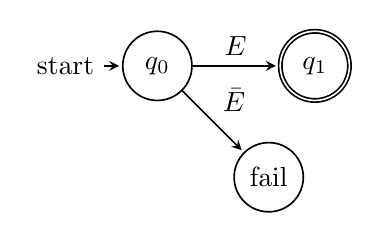
\begin{tikzpicture}[->,shorten >=1pt,node distance=2cm,on
      grid,auto,scale=.5,semithick,>=stealth]
			\node[state,initial] (q0) {$q_0$};
			\node[state,accepting] (q1) [right of=q0] {$q_1$};
			\node[state] (fail) [below right of=q0] {fail};
			\path
				(q0) edge node {$E$} (q1)
        (q0) edge node {$\bar{E}$} (fail);
		\end{tikzpicture}
    \subcaption{The \textit{assert} specification.}
	\end{minipage}
  ~
	\begin{minipage}{0.45\textwidth}
		\centering
		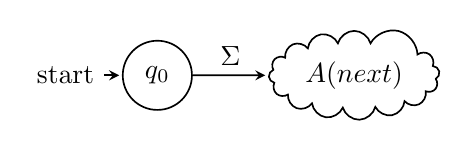
\begin{tikzpicture}[->,shorten >=1pt,node distance=2.5cm,on
      grid,auto,scale=.5,semithick,>=stealth]
			\node[state,initial] (q0)	{$q_0$};
			\node[cloud, cloud puffs=15.7, cloud ignores aspect, align=center, draw] (cloud) [right of=q0] {$A(next)$};
			\path
				(q0) edge node {$\Sigma$} (cloud);
		\end{tikzpicture}
    \subcaption{The \textit{next} specification.}
	\end{minipage}

  \bigskip

	\begin{minipage}{0.90\textwidth}
		\centering
		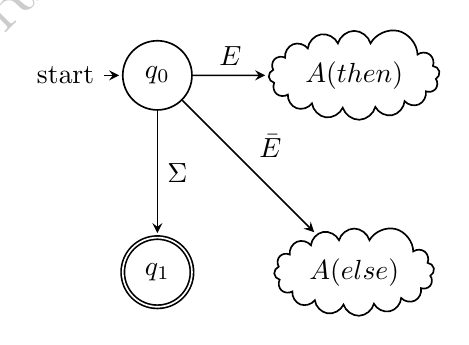
\begin{tikzpicture}[->,shorten >=1pt,node distance=2.5cm,on
      grid,auto,scale=.5,semithick,>=stealth]
			\node[state,initial] (q0)	{$q_0$};
			\node[cloud, cloud puffs=15.7, cloud ignores aspect, align=center, draw] (then) [right of=q0] {$A(then)$};
			\node[cloud, cloud puffs=15.7, cloud ignores aspect, align=center, draw] (else) [below of=then] {$A(else)$};
			\node[state,accepting] (q1) [below of=q0]	{$q_1$};
			\path
				(q0) edge node {$E$} (then)
        (q0) edge node {$\bar{E}$} (else)
        (q0) edge node {$\Sigma$} (q1);
		\end{tikzpicture}
    \subcaption{The \textit{if} specification.}
	\end{minipage}

  \caption{Sketches of automata for the three basic formal specification
    functions. The squiggles around $A(next)$, $A(then)$ and $A(else)$ denote
    that some composition is required there.}
	\label{figure-basic-formal-specification-automata}
\end{figure}
%%%%%%%%%%%%%%%%%%%%%%%%
%%%%%%%%%%%%%%%%%%%%%%%%
%%%%%%%%%%%%%%%%%%%%%%%%


\subsection{Rules for Composition} \label{section-approach-composition}
\lstset{language=Python,numbers=none}

The idea is to use composition to build more complex and interesting
specifications from the three basic formal specification functions. Composition
is defined formally, which preserves the semantics from
section~\ref{section-approach-semantics}.

There are no implicit precedence rules for the $\circ$ composition operator;
parentheses are required.


\subsubsection{Composition of the \textit{assert} specification, and
composition with the \textit{tail} composition point}

The \textit{assert} specifications are the only basic formal specification
functions that are complete, without the need to compose them with other
specifications. The automata $A(a_E)$ for a standalone \textit{assert}
specification $a_E$, shown in
Figure~\ref{figure-basic-formal-specification-automata}, is defined as:

\[
  \begin{array}{rcl}
    A(a_E) & = & (\{q_0, q_1, f\}, \{(q_0, q_1, E), (q_0, f, \bar{E})\}, q_0, \{q_1\})
  \end{array}
\]

$f$ (\textit{fail}) is a failure state, from which no transitions lead. If
$\bar{E}$ is true, the failure state will be reached, and no further
verification can be done.

\textit{assert} specifications, and all formal specification functions, have at
least one open composition point, the \textit{tail} composition point.
Compositions using the \textit{tail} composition point are commutative: $s \,
\circ_{tail} \, s' = s' \, \circ_{tail} \, s$. Composition using the
\textit{tail} composition point is essentially just a merge of the initial
states of the two specifications, making the initial transitions of both
specifications go out from the same state $q_0$, and merging the accepting
states of the automata. Given two specifications $s$ and $s'$, where:

\medskip
\[
  \begin{array}{rcl}
    A(s) & = & (Q_s, T_s \cup P_s, q_{0s}, F_s) \\
   A(s') & = & (Q_{s'}, T_{s'} \cup P_{s'}, q_{0s'}, F_s \cup F_{s'})
  \end{array}
\]
\medskip

Then:

\medskip
\[
  \begin{array}{rcl}
    A(s \circ_{tail} s') & = & (\{q_0\} \cup Q_s \cup Q_{s'} - \{q_{0s}, q_{0s'}\}, T \cup (P_s \cup P_{s'}), q_0, F_{s'}) \\
                     T   & = & \{(q_0, q', E) \, | \, (q, q', E) \in (T_s \cup T_{s'})\}
  \end{array}
\]
\medskip

An example is shown for two \textit{assert} specifications in
Figure~\ref{figure-assert-composition-example}. The resulting automata is
unnecessarily complex, and can be simplified to a smaller automata with the
same semantics, as seen in Figure~\ref{figure-assert-composition-simplified}.


%%%%%%%%%%%%%%%%%%%%%%%%
%% Composition, assert o s, symbol-python-automata
%%%%%%%%%%%%%%%%%%%%%%%%
\begin{figure}[h!]
	\begin{minipage}{0.90\textwidth}
		\centering
    \[
      \begin{array}{rcl}
        A(a_E) & = & (\{q_x, q_y, f\}, \{(q_x, q_y, E), (q_x, f, \bar{E})\}, q_x, \{q_y\}) \\
    A(a'_{E'}) & = & (\{q_z, q_w, f'\}, \{(q_z, q_w, E') ,(q_z, f', \bar{E'})\}, q_z, \{q_w\})
      \end{array}
    \]
		\centering
    \[
      \begin{array}{rcl}
        A(a_E \circ_{tail} a'_{E'}) & = & (Q, P, q_0, F) \\
                                 Q & = & \{q_0, q_y, f, q_w, f'\} \\
                                 P & = & \{(q_0, q_y, E), (q_0, f, \bar{E}), (q_0, q_w, E), (q_0, f', \bar{E'})\} \\
                                 F & = & \{q_y, q_w\}
      \end{array}
    \]
	\end{minipage}

  \bigskip

	\begin{minipage}{0.45\textwidth}
		\centering
    \begin{lstlisting}
def s(event):
  assert E
  assert E'
    \end{lstlisting}
	\end{minipage}
  ~
	\begin{minipage}{0.45\textwidth}
		\centering
		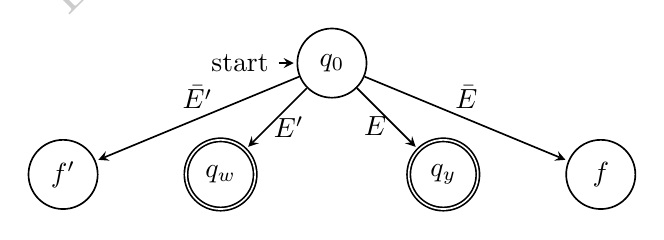
\begin{tikzpicture}[->,shorten >=1pt,node distance=2cm,on
      grid,auto,scale=.5,semithick,>=stealth]
			\node[state,initial] (q0) {$q_0$};
			\node[state,accepting] (qy) [below right of=q0] {$q_y$};
			\node[state] (f) [right of=qy] {$f$};
			\node[state,accepting] (qw) [below left of=q0] {$q_w$};
			\node[state] (f') [left of=qw] {$f'$};
			\path
        (q0) edge node [pos=0.3, below] {$E$} (qy)
        (q0) edge node [pos=0.3, below] {$E'$} (qw)
        (q0) edge node [above] {$\bar{E}$} (f)
        (q0) edge node [pos=0.5, above] {$\bar{E'}$} (f');
		\end{tikzpicture}
	\end{minipage}
  \caption{An example showing a composition of an \textit{assert} specification
    $a_E$ with another \textit{assert} specification $a'_{E'}$. Only the
    resulting $A(a_E \, \circ_{tail} \, a'_{E'})$ automata is shown.}
	\label{figure-assert-composition-example}
\end{figure}

\begin{figure}[h!]
	\begin{minipage}{0.45\textwidth}
		\centering
    \[
      (\{q_0, q_1, f\}, \{(q_0, q_1, E \wedge E'), (q_0, f, \bar{E} \vee \bar{E'})\}, q_0, \{q_1\})
    \]
	\end{minipage}
	\begin{minipage}{0.45\textwidth}
		\centering
		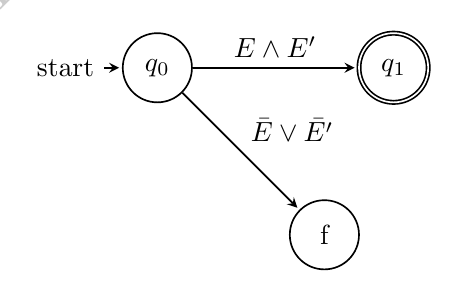
\begin{tikzpicture}[->,shorten >=1pt,node distance=3cm,on
      grid,auto,scale=.5,semithick,>=stealth]
			\node[state,initial] (q0) {$q_0$};
			\node[state,accepting] (q1) [right of=q0] {$q_1$};
			\node[state] (f) [below right of=q0] {f};
			\path
				(q0) edge node {$E \wedge E'$} (q1)
        (q0) edge node {$\bar{E} \vee \bar{E'}$} (f);
		\end{tikzpicture}
	\end{minipage}
  \caption{A simplified version of the automata from
    Figure~\ref{figure-assert-composition-example}, semantically identical.}
	\label{figure-assert-composition-simplified}
\end{figure}

%%%%%%%%%%%%%%%%%%%%%%%%
%%%%%%%%%%%%%%%%%%%%%%%%
%%%%%%%%%%%%%%%%%%%%%%%%


\subsubsection{Composition of the \textit{next} specification}

\textit{next} specifications have two composition points: one appropriately
called \textit{next}, which is required, and one called \textit{tail}, which
is optional. Composition using the \textit{tail} composition point was
described above.

Composition with the \textit{next} composition point, $n \, \circ_{next} \, s$
with $A(s) = (Q, P, q_0, F)$ is as follows:

\[
  \begin{array}{rcl}
    A(n \circ_{next} s) & = & (\{q_0'\} \cup Q, T \cup P, q_0', F) \\
               T  & = & \{(q_0', q_0, \Sigma)\}
  \end{array}
\]

This is illustrated in Figure~\ref{figure-next-composition-s}.

Also note that composition using the \textit{next} composition point is
associative, as shown in Figure~\ref{figure-next-associative}.



%%%%%%%%%%%%%%%%%%%%%%%%
%% Composition, next o s, symbol-python-automata
%% Associativity of the next composition point
%%%%%%%%%%%%%%%%%%%%%%%%
\begin{figure}[h!]
	\begin{minipage}{0.25\textwidth}
		\centering
    \[
      s' = n \, \circ_{next} \, s
    \]
	\end{minipage}
  ~
	\begin{minipage}{0.25\textwidth}
		\centering
    \begin{lstlisting}
def s'(event):
  event.next(s)
    \end{lstlisting}
	\end{minipage}
  ~
	\begin{minipage}{0.4\textwidth}
		\centering
		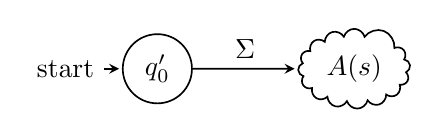
\begin{tikzpicture}[->,shorten >=1pt,node distance=2.5cm,on
      grid,auto,scale=.5,semithick,>=stealth]
			\node[state,initial] (q0')	{$q_0'$};
			\node[cloud, cloud puffs=15.7, cloud ignores aspect, align=center, draw] (cloud) [right of=q0'] {$A(s)$};
			\path
				(q0') edge node {$\Sigma$} (cloud);
		\end{tikzpicture}
	\end{minipage}
  \caption{A composition of a \textit{next} specification and an
    \textit{assert} specification, with the \textit{next} specification on the
    left-hand side.}
	\label{figure-next-composition-s}
\end{figure}

\begin{figure}[h!]
	\begin{minipage}{0.9\textwidth}
		\centering
    \[
      \begin{array}{rcl}
        (n \, \circ_{next} \, s_1) \, \circ_{tail} \, (n' \, \circ_{next} \, s_2)
        & = & n \, \circ_{next} \, t \\
        t & = & s_1 \, \circ_{tail} \, s_2
      \end{array}
    \]
	\end{minipage}

  \bigskip

	\begin{minipage}{0.45\textwidth}
		\centering
    \begin{lstlisting}
def s(event):
  event.next(s1)
  event.next(s2)

# equivalent to
def s(event):
  event.next(t)

def t(event):
  s1()
  s2()
    \end{lstlisting}
	\end{minipage}
  ~
	\begin{minipage}{0.45\textwidth}
		\centering
		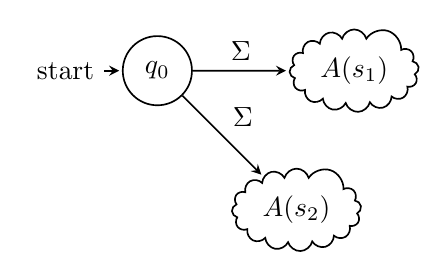
\begin{tikzpicture}[->,shorten >=1pt,node distance=2.5cm,on
      grid,auto,scale=.5,semithick,>=stealth]
			\node[state,initial] (q0)	{$q_0$};
			\node[cloud, cloud puffs=15.7, cloud ignores aspect, align=center, draw] (s1) [right of=q0] {$A(s_1)$};
			\node[cloud, cloud puffs=15.7, cloud ignores aspect, align=center, draw] (s2) [below right of=q0] {$A(s_2)$};
			\path
				(q0) edge node {$\Sigma$} (s1)
				(q0) edge node {$\Sigma$} (s2);
		\end{tikzpicture}

    \bigskip

		\centering
		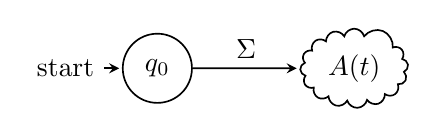
\begin{tikzpicture}[->,shorten >=1pt,node distance=2.5cm,on
      grid,auto,scale=.5,semithick,>=stealth]
			\node[state,initial] (q0) {$q_0$};
			\node[cloud, cloud puffs=15.7, cloud ignores aspect, align=center, draw] (t) [right of=q0] {$A(t)$};
			\path
				(q0) edge node {$\Sigma$} (t);
		\end{tikzpicture}
	\end{minipage}
  \caption{The associativity of the \textit{next} composition point in a
  \textit{next} formal specification function.}
	\label{figure-next-associative}
\end{figure}
%%%%%%%%%%%%%%%%%%%%%%%%
%%%%%%%%%%%%%%%%%%%%%%%%
%%%%%%%%%%%%%%%%%%%%%%%%


\subsubsection{Composition of the \textit{if} specification}

\textit{if} specifications have three composition points: \textit{then}, which
is required, and two optional, \textit{else} and \textit{tail}. Composition
using the \textit{tail} composition point was described above.

In an \textit{if} specification $i_E$ we consider the expression $E$ as a guard
for the \textit{then} composition point, $\bar{E}$ as a guard for the
\textit{else} composition point.

The composition then becomes essentially to add the guard $E$ to the labels of
all initial transitions for the automata at the \textit{then} composition
point, and $\bar{E}$ to the labels of all initial transitions fro the automata
at the \textit{else} composition point. The guards, $E$ and $\bar{E}$ are added
as parts of a conjunctive.

Let $s_1$ be the specification attached to the \textit{then} composition point
and an optional $s_2$ attached to the \textit{else} composition point, and
$A(s_1) = (Q_1, T_1 \cup R_1, q_{10}, F_1)$, $A(s_2) = (Q_2, T_2 \cup R_2,
q_{20}, F_2)$. Then:

\[
  \begin{array}{rcl}
  A((i_E \circ_{then} s_1) \circ_{else} s_2) & = & (Q \cup \{q_0, q_1\}, T_1 \cup T_2 \cup X \cup R, q_0, F \cup \{q_1\}) \\
                                        T_1  & = & \{(q_0, q, E       \wedge E') \, | \, (q_{10}, q, E') \in T_1\} \\
                                        T_2  & = & \{(q_0, q, \bar{E} \wedge E') \, | \, (q_{20}, q, E') \in T_2\} \\
                                         X   & = & \{(q_0, q_1, \Sigma)\}
  \end{array}
\]

If $s_2$ is left out, a dummy \textit{assert} specification of the form
\texttt{assert True} is inserted instead, which would mean $A(s_2) =
(\{a,b\}, (a, b, \Sigma), a, \{b\})$.

The fall-through to the \textit{tail} composition point is represented by the
$X$ transition.

%%%%%%%%%%%%%%%%%%%%%%%%
%% Composition, if o s, symbol-python-automata
%%%%%%%%%%%%%%%%%%%%%%%%
%%%%%%%%%%%%%%%%%%%%%%%%
%%%%%%%%%%%%%%%%%%%%%%%%
%%%%%%%%%%%%%%%%%%%%%%%%








%================================================
%====== Chapter 5, Evaluation
%================================================

\pagestyle{newchap}
\chapter{Evaluation} \label{chapter-evaluation}

To see how \textit{pythonrv} would work in a real-world setting it was
incorporated into a real-time web application for Valtech Sweden, a
medium-sized Swedish company.

The web application is written in Python 2.7 using the
Django\footnote{\texttt{https://www.djangoproject.com/}} web framework. It has
approximately 10000 lines of code.

There are two questions we need to answer when writing specifications for a
program. First, when, in the life-cycle of the program, should we attach the
specifications? I.e.\ when should the code instrumentation be done? And second,
and most important: what specifications should be written, and for which
functions?

We can answer the first question first. It requires a bit of knowledge on the
start up sequence for, and structure of, Django applications.


\section{Technical Perspective}


\subsection{Anatomy of a Django Application}

A Django application follows the Model-View-Controller
pattern\footnote{\todo{Link somewhere?}}, or as they call it, the
Model-Template-View pattern. The model is a representation of the data used by
the program, and the templates are the layer that constructs the display for
the user. The view links the two together, fetching the correct models for
specific requests, and then delegating to the appropriate templates.

Application-specific configuration for Django programs are stored in settings
modules, which are ordinary Python files. These contain settings for database
connections, authentication, etc.. During startup, Django reads the settings
files, starts up its internal machinery, and waits for the first request.


\subsection{When to Attach}

At first glance it might seem desirable to attach the specifications before
even starting the Django framework. That way we could monitor the startup
process, and all of the functionality of Django.

A problem with this, that is due to how Python works, and how \textit{pythonrv}
does code instrumentation, is that \textit{pythonrv} needs to load the modules
(files) for each function to be monitored. These modules are often heavily
dependent on Django, and that it has been started correctly, with all settings
loaded.

A suitable time to instrument the program - to enable the specifications - is
during startup, after the settings have been loaded. Some specifications, which
do not monitor code dependent on the settings, could be loaded before that.


\subsection{Issues}

Early in the process of using \textit{pythonrv} in the program it was
discovered that the copying of data, such as function arguments, that
\textit{pythonrv} does would not work with Django. The latest version of
Django, v1.4.1, uses a module called \texttt{cStringIO}, which produces objects
that cannot be copied. All functions dealing with web requests are affected by
this. This has been fixed in the development branch of Django, but in the
meantime, \textit{pythonrv} has an option to disable argument copying, either
for all specifications or for a subset of them, to work around this issue.


\section{Potential Value}

Now to the most important question: what specifications could, and should, be
written? What value do they provide?

\todo{}
Talk about where specifications would be suitable, and for what.




%================================================
%====== Chapter 6, Conclusions
%================================================

\pagestyle{newchap}
\chapter{Conclusions} \label{chapter-conclusions}

This report, and the proof-of-concept implementation \textit{pythonrv}, has
shown that it is possible to write specifications in the target programs
programming language (Python) and in a manner more similar to unit testing.

However, a few reservations should be mentioned. The specification functions'
explicit dealing with time and the actual execution flow leads to some inherent
divergences from ordinary unit testing styles.

Also, giving the specifications a formal foundation, and doing formal
verification with them, is different, and perhaps more difficult, than with
specifications already written in formal languages. The fact that the chosen
programming language, Python, does not have a formal semantics defined makes the
task quite a bit larger.

The formal foundation given in section~\ref{section-approach-formal-foundation}
is thus for a small subset of Python, which makes the math easier, but the
resulting semantics less interesting.

If the verification parts of \textit{pythonrv} is unwanted, it could be used as
a simple framework for aspect-oriented programming.

\section{Future Work}

The testing tool called expectations, as described in
Chapter~\ref{chapter-previous-research} could fit quite well with the
\textit{pythonrv} style of writing specifications.

The performance of the implementation has not been measured or considered in
much detail. Benchmark tests for \textit{pythonrv} would be interesting, as
would attempts to introduce it as a correctness verification approach for more
programs.

Offline verification, discussed in Section~\ref{section-rv} and
Section~\ref{section-approach-verification} would be interesting.

\section{Discussion}

The trend of software systems in general seems to be toward larger and more
complex entities. This makes the automated verification of program
correctness, formal or not, ever more important and an essential part of
software development. Runtime verification could have a place there, if it
becomes more popular and simpler to integrate and use in ordinary software.

The implementation described in this report, \textit{pythonrv}, is publicly
available on the web\footnote{\texttt{https://github.com/tgwizard/pythonrv}} as
free, open source software. People are welcome to try it, incorporate it into
their programs, and extend it, as they see fit. With enough interest,
\textit{pythonrv} might develop into a mature framework for runtime
verification.




%================================================
%====== Bibliography
%================================================

% the ieeetr style orders the references after first appearance
\bibliographystyle{ieeetr}
\bibliography{references}




%================================================
%====== Appendices
%================================================

% no appendices yet

\end{document}
